\section{Results}

The present study investigated the differences in gaze-based strategies dependent on task, tool familiarity, and handle orientation. Here, we investigated two anticipatory gaze-based strategies 3 seconds before action initiation; the odds of fixations in favor of the tool effector and the eccentricity of the fixations through time towards the tool effector. We further compared the differences in two experiments that had the same experimental design but differed in the realism of the action affordance and environment. 


\begin{figure}[t]
    \centering
    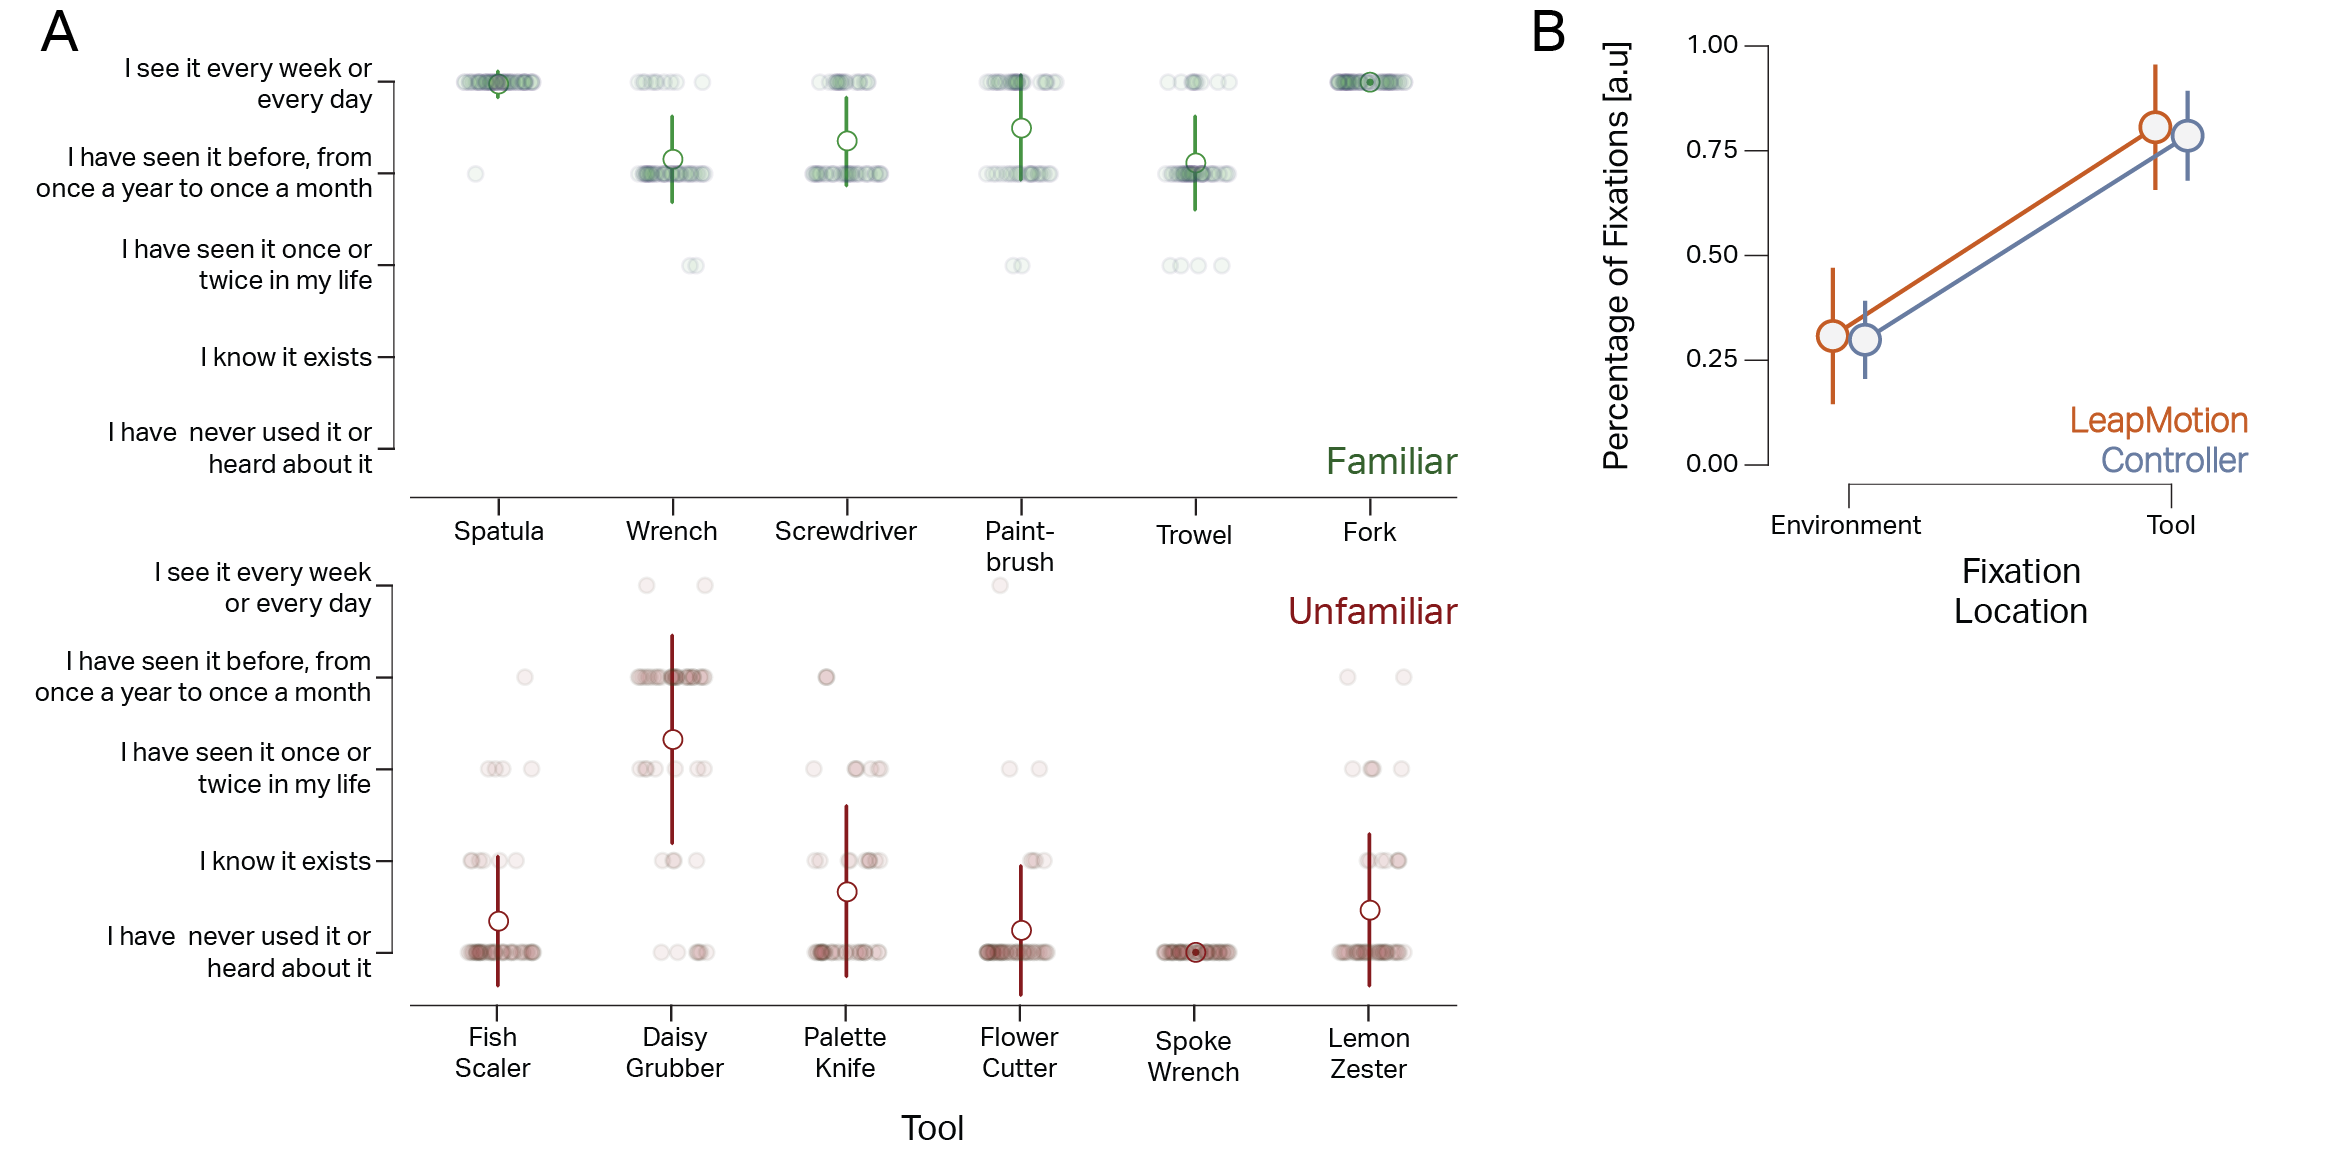
\includegraphics[width=1\linewidth]{source/figures/result/results_exp_comp.png} \\
    \caption[]{ \textbf{A)}  Participants’ familiarity rating of the tools. Participants provided their subjective rating of familiarity with the 12 tool stimuli on a 5-point Likert scale. The small circles correspond to ratings from individual subjects. The larger circles correspond to the mean rating for each tool, and error bars represent the standard deviation across subjects. \textbf{B)} Percentage of fixations allocated to the environment vs. the tools for the two different experiments. The circles correspond to the mean percentage of fixations across subjects, and the error bars represent the standard deviation. As seen here, the realism of the environment did not affect how participants allocated their attention in the experiments. }
    \label{figure:familiarity_rating}
\end{figure}

First, we were interested in how the participants subjectively assessed the familiarity of the 12 tools. \ref{figure:familiarity_rating}A shows the subjective familiarity ratings for each of the familiar and unfamiliar tools used in the study. The mean familiarity rating for familiar tools in experiment-I was 4.55 (SD=0.60) and for unfamiliar tools 1.81 (SD=1.17). In experiment-II, the mean familiarity rating for familiar tools was 4.48 (SD=0.52) and for unfamiliar tools 1.56 (SD=1.04). To determine the differences in the subjective familiarity ratings for the two experiments and our categorization of familiarity, we performed a mixed-ANOVA with familiarity as a within-subject factor and the experiment group as the between-subject factor. We found no differences in the familiarity ratings between the two experiments (F(44)=3.08, p-value=0.08). Furthermore, there were significant differences in the subjective rating of the tools (F(44)=3094.05, p-value<0.001). There were also no significant interactions between the two factors (F(44)=2.52, p-value=0.11). Figure  In sum, our experimental condition of familiarity was consistent with the participants’ subjective rating as well. 

Next, we wanted to make sure that the differences in the virtual environments did not affect the way subjects allocated their attention to the experimental task. We calculated the mean percentage of fixations positioned on the tool vs. anywhere else in the environment for each subject across trials. Figure \ref{figure:familiarity_rating}B shows the percentage of fixations allocated to the tools vs. the environment for the two experiments. For experiment-I with the interaction method of VR controller and a less realistic environment, the mean percentage of fixations on the environment was 0.29 (SD=0.08) and on the tools 0.78 (SD=0.10). Conversely, in experiment-II with LeapMotion as the interaction method and a more realistic environment, the percentage of fixations allocated to the environment was 0.30 (SD=0.15) and on the tools 0.80 (SD=0.14). To test if these differences were significant, we performed a mixed-ANOVA with fixation location as a within-subject factor, the two experiments as a between-subject factor, and the percentage of fixations as the dependent variable.  We found no differences in the percentage of fixations between the two experiments (F(47)=2.86, p-value=0.09). There were significant differences in the percentage of fixations located on the tool vs. the environment (F(47)=217.47, p-value<0.001). We did not find any interactions between the two factors (F(47)=0.02, p-value=0.87). These results show that the allocation of attention was primarily task-oriented and was not affected by the differences in the virtual environment of the two experiments.

\begin{figure}[h]
    \centering
    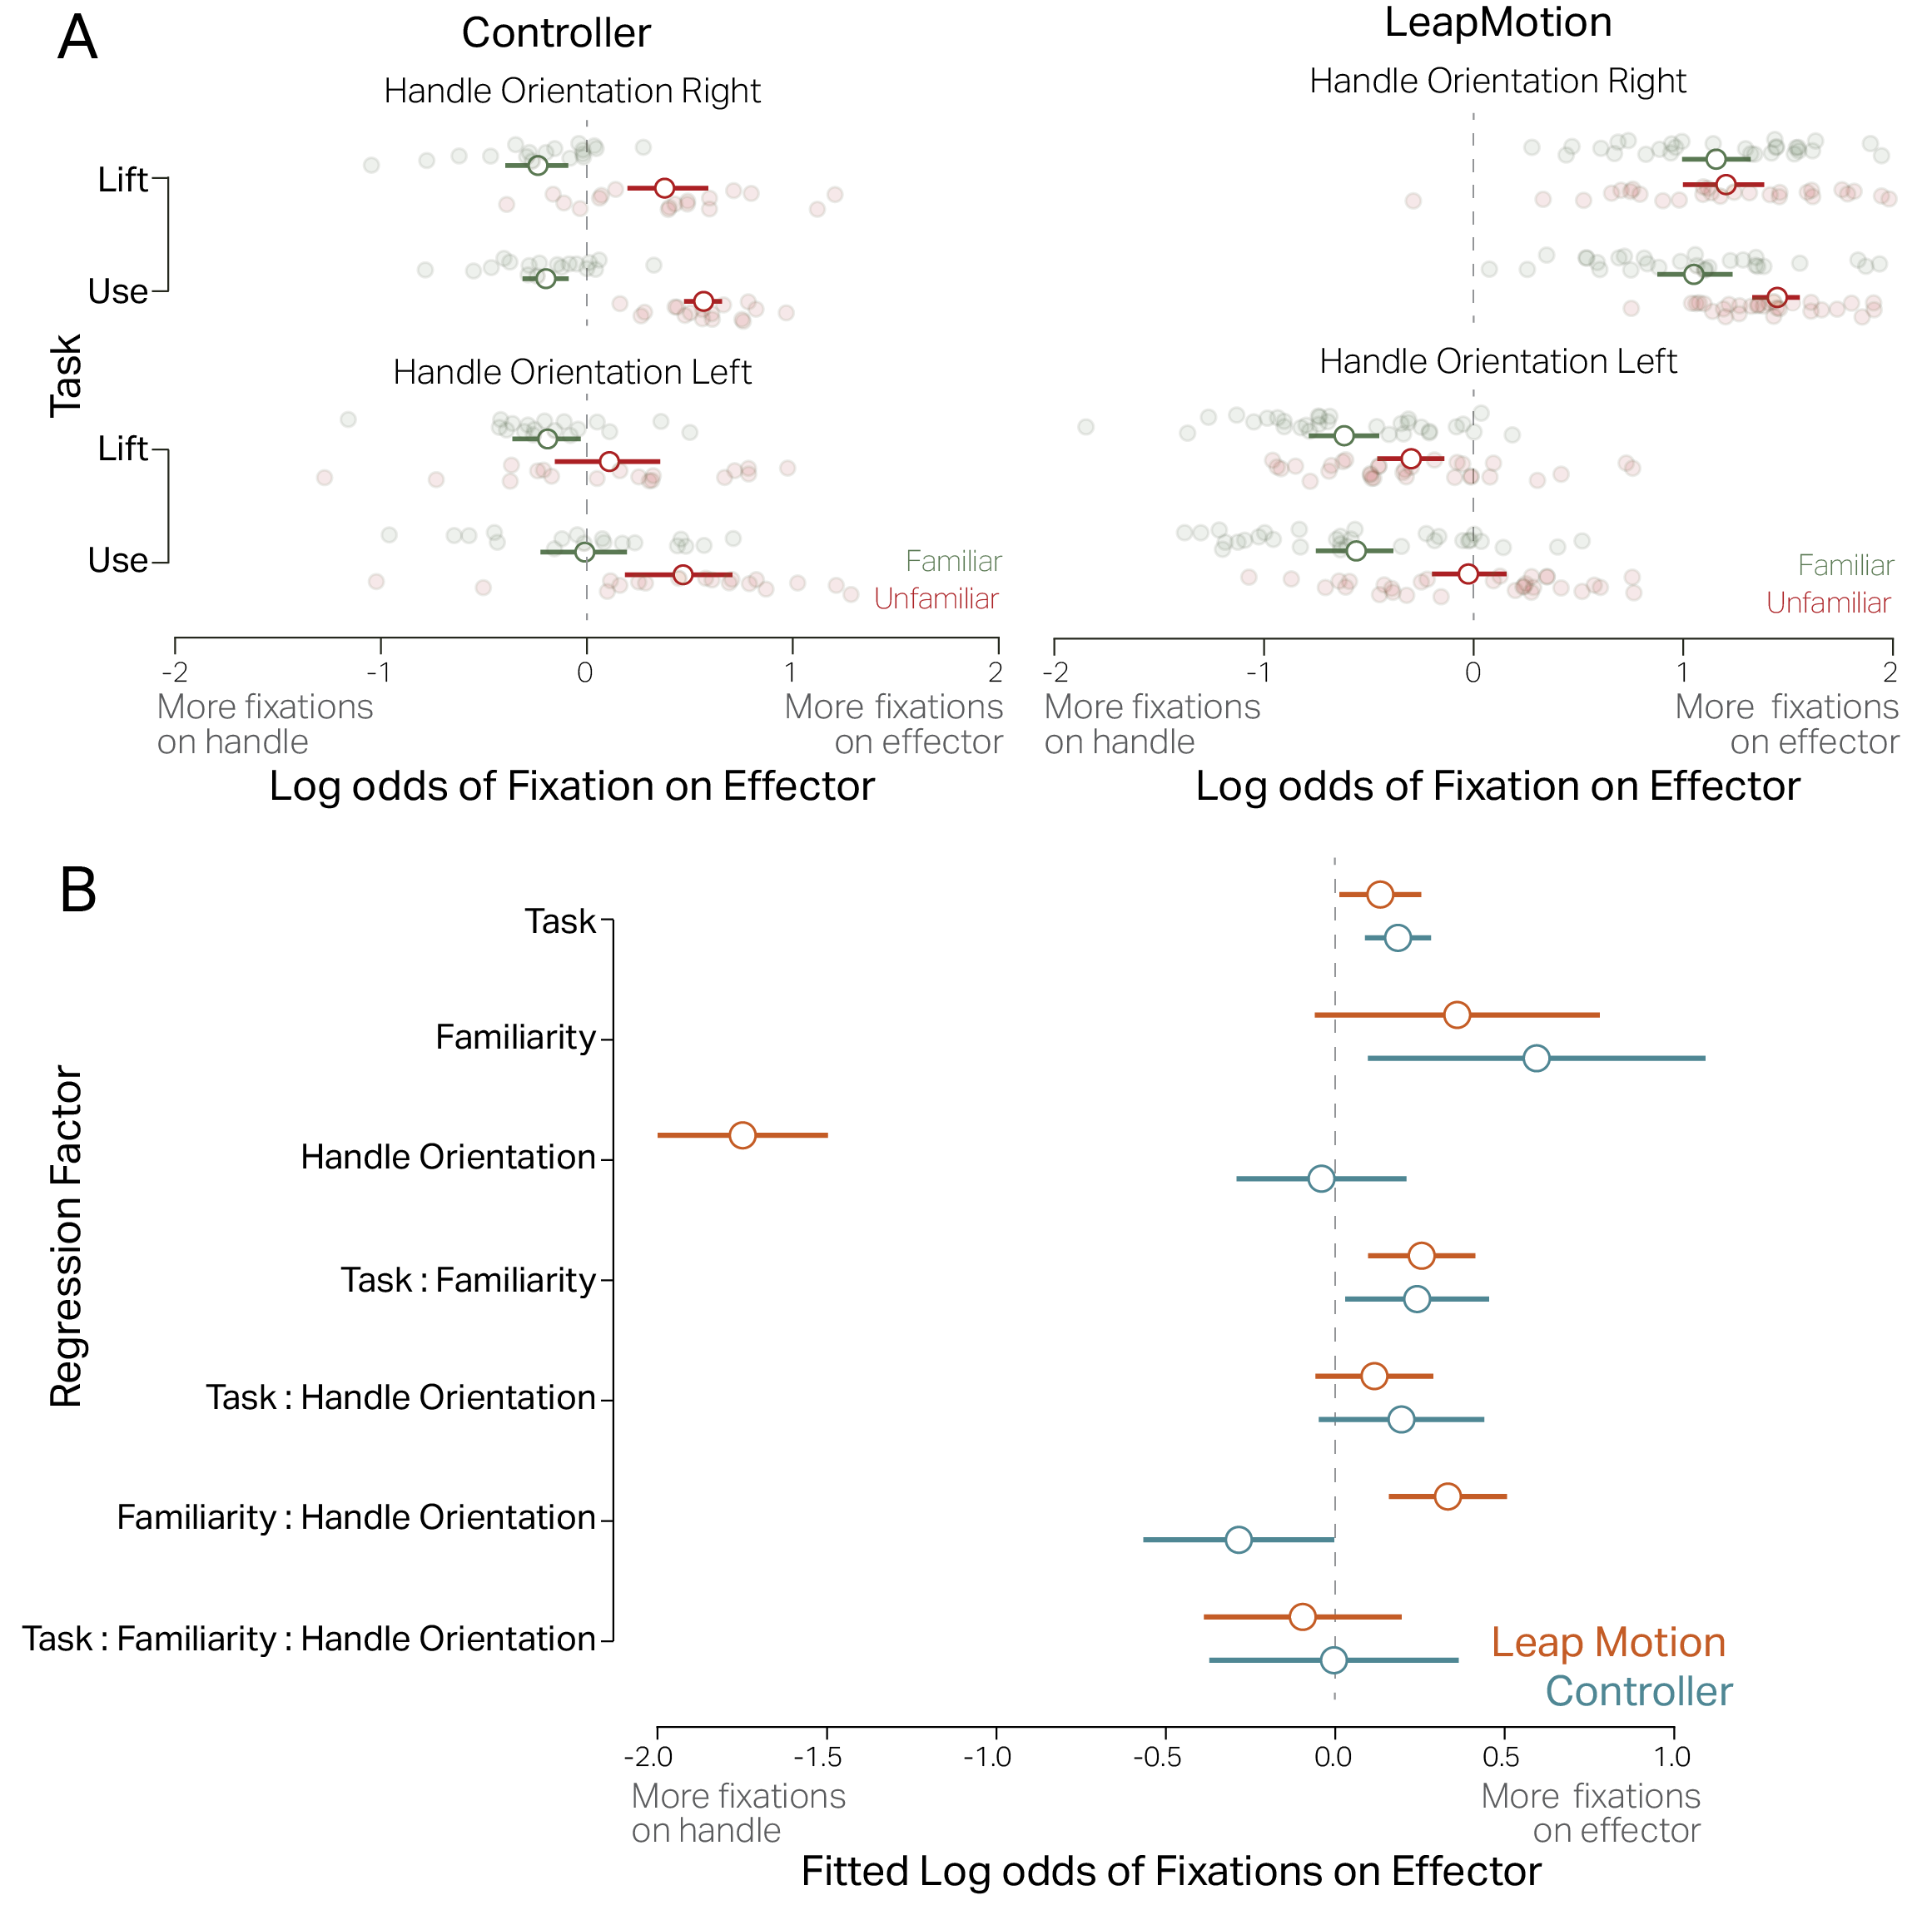
\includegraphics[width=0.9\linewidth]{source/figures/result/results_combined_logodds_fullmodel.png} \\
    \caption[]{Experiment results. \textbf{A)} \textbf{top-left:} shows the log-odds of fixation on effector vs. handle in the controller study when the tool handle is oriented to the right. The log odds on fixations are higher on the effector for unfamiliar tools (red) than the familiar tools (green) for both the LIFT and the USE tasks. \textbf{Bottom-left:} log odds of fixation on effector when the tool handle is oriented to the left and is incongruent to the subjects’ handedness. The plot shows that the orientation of the tool does not significantly affect the log-odds fixation on the effector. \textbf{Top-right:} the log-odds of fixation on effector in the LeapMotion study when the tool handle is oriented to the right. The log odds of fixations on the effector are higher for unfamiliar tools (red) than the familiar tools (green) and the USE task. \textbf{Bottom-right:} log odds of fixation on effector when the tool handle is oriented to the left and is incongruent to the subjects’ handedness. The plot shows that the orientation of the tool results in significant log-odds of fixations over the handle in the LIFT task, while in the USE task and with unfamiliar tools (red) significantly more fixations were on the effector. \textbf{B)} The linear regression coefficients for the two experiments. The effect of the task is significant for both experiments with higher log-odds of fixations on the effector. For the factor orientation, the log-odds are significant in the LeapMotion experiment and not for the controller experiment. Similarly, the interaction between task and familiarity is significant for both experiments.
}
    \label{figure:log_odds}
\end{figure}


Next, we compared the log-odds of fixations in favor of the tool effector across the three conditions: task, tool familiarity, and handle orientation in the 3s period when the subjects studied the tool. Figure 3A shows the log-odds of the fixations on the tool effector for experiment-I (with HTC VIVE Controllers) and experiment-II (with LeapMotion). In experiment-I (Figure \ref{figure:log_odds}A, left panel), subjects showed a mean log odds of 0.01 (95\%CI = [-0.04, 0.08]) for the LIFT task and for the USE task the mean log-odds were 0.19 (95\%CI = [0.11, 0.28]). For the FAMILIAR tools, the mean log-odds in favor of the tool effector were -0.16 (95\%CI = [-0.23, -0.09]) and for UNFAMILIAR 0.35 (95\%CI = [0.25, 0.45]). For the  RIGHT oriented tool handle, the mean log-odds were 0.14 (95\%CI = [0.06, 0.21]) and for the LEFT oriented tool handle, the mean log-odds were 0.08 (95\%CI = [-0.09, 0.26]). To assess the significance of the factors, we used linear mixed models. For the linear model, we used effect coding so the regression coefficients can be directly interpreted as main effects. There was a significant main effect of factor task (USE - LIFT) $\beta$ = 0.18 (95\%CI = [0.08, 0.27], t(70.09)=3.7), with a p-value < 0.001. There was a significant main effect of familiarity (UNFAMILIAR - FAMILIAR ) $\beta$ = 0.58  (95\%CI = [0.09, 1.08], t(10.79)=2.33), with p-value = 0.04. The main effect of handle orientation was not significant (LEFT - RIGHT) $\beta$ = -0.04, (95\%CI = [-0.29, 0.21], t(16.94)=-0.32), p-value = 0.75. We found a significant interaction of task and familiarity with $\beta$ = 0.24  (95\%CI = [0.03, 0.45], t(25.88)=2.21), p-value = 0.036. The interaction of task and handle orientation was not significant, $\beta$ = 0.19  (95\%CI = [-0.05, 0.43], t(21.26)=1.55), p-value = 0.13. The interaction of familiarity and orientation was not significant , $\beta$ = -0.28  (95\%CI = [-0.56, -0.004], t(17.07)=-1.99), p-value = 0.06. The 3-way interaction was also not significant, $\beta$ = -0.005  (95\%CI = [-0.37, 0.36], t(1695)=-0.02), p-value=0.97.

In experiment-II (Figure \ref{figure:log_odds}A, right panel), subjects showed a mean log odds of 0.08 (95\%CI = [-0.04, 0.22]) of fixations on the tool effector for the LIFT task and for the USE task the mean log-odds were 0.22 (95\%CI = [0.09, 0.36]). For the FAMILIAR tools, the mean log-odds in favor of the tool effector were 0.04 (95\%CI = [-0.08, 0.16]) and for UNFAMILIAR 0.25 (95\%CI = [0.12, 0.39]). For the RIGHT oriented tool handle, the mean log-odds were 1.18 (95\%CI = [1.06, 1.29]) and for the LEFT oriented tool handle, the mean log-odds were -0.32 (95\%CI = [-0.45, -0.20]).  Using the linear mixed model, we assessed the significance of the three factors. There was a significant main effect of factor task (USE - LIFT) $\beta$ = 0.13  (95\%CI = [0.01, 0.25], t(27.28)=2.13) with a p-value = 0.04. The main effect of familiarity (UNFAMILIAR - FAMILIAR ) was not significant $\beta$ = 0.35  (95\%CI = [-0.06, 0.77], t(10.02)=1.67) with p-value = 0.12. The main effect of handle orientation (LEFT - RIGHT) was significant, $\beta$ = -1.74 (95\%CI = [-1.99, -1.48], t(28)=-13.65), p-value <0.001. We found a significant interaction of task and familiarity with $\beta$ = 0.25 (95\%CI = [0.09, 0.41], t(43.64)=3.13), p-value = 0.003. The interaction of task and handle orientation was not significant, $\beta$ = 0.11 (95\%CI = [-0.06, 0.28], t(31.90)=1.29), p-value = 0.20. Similarly, the interaction of familiarity and orientation was significant, $\beta$ = 0.33 (95\%CI = [0.15, 0.50]), p-value = 0.001. The 3-way interaction was also not significant, $\beta$ = -0.09 (95\%CI = [-0.39, 0.19], t(2201)=-0.65), p-value=0.51.

Figure \ref{figure:log_odds}B summarizes the regression coefficients of the linear model from both experiments. Importantly, we see that the main effect of the task is significant for both experiments. Similarly, the interaction of task and familiarity is significant for both experiments. However, the effect of handle orientation is only significant in experiment-II with the LeapMotion interaction method. 

\begin{figure}[ht]
    \centering
    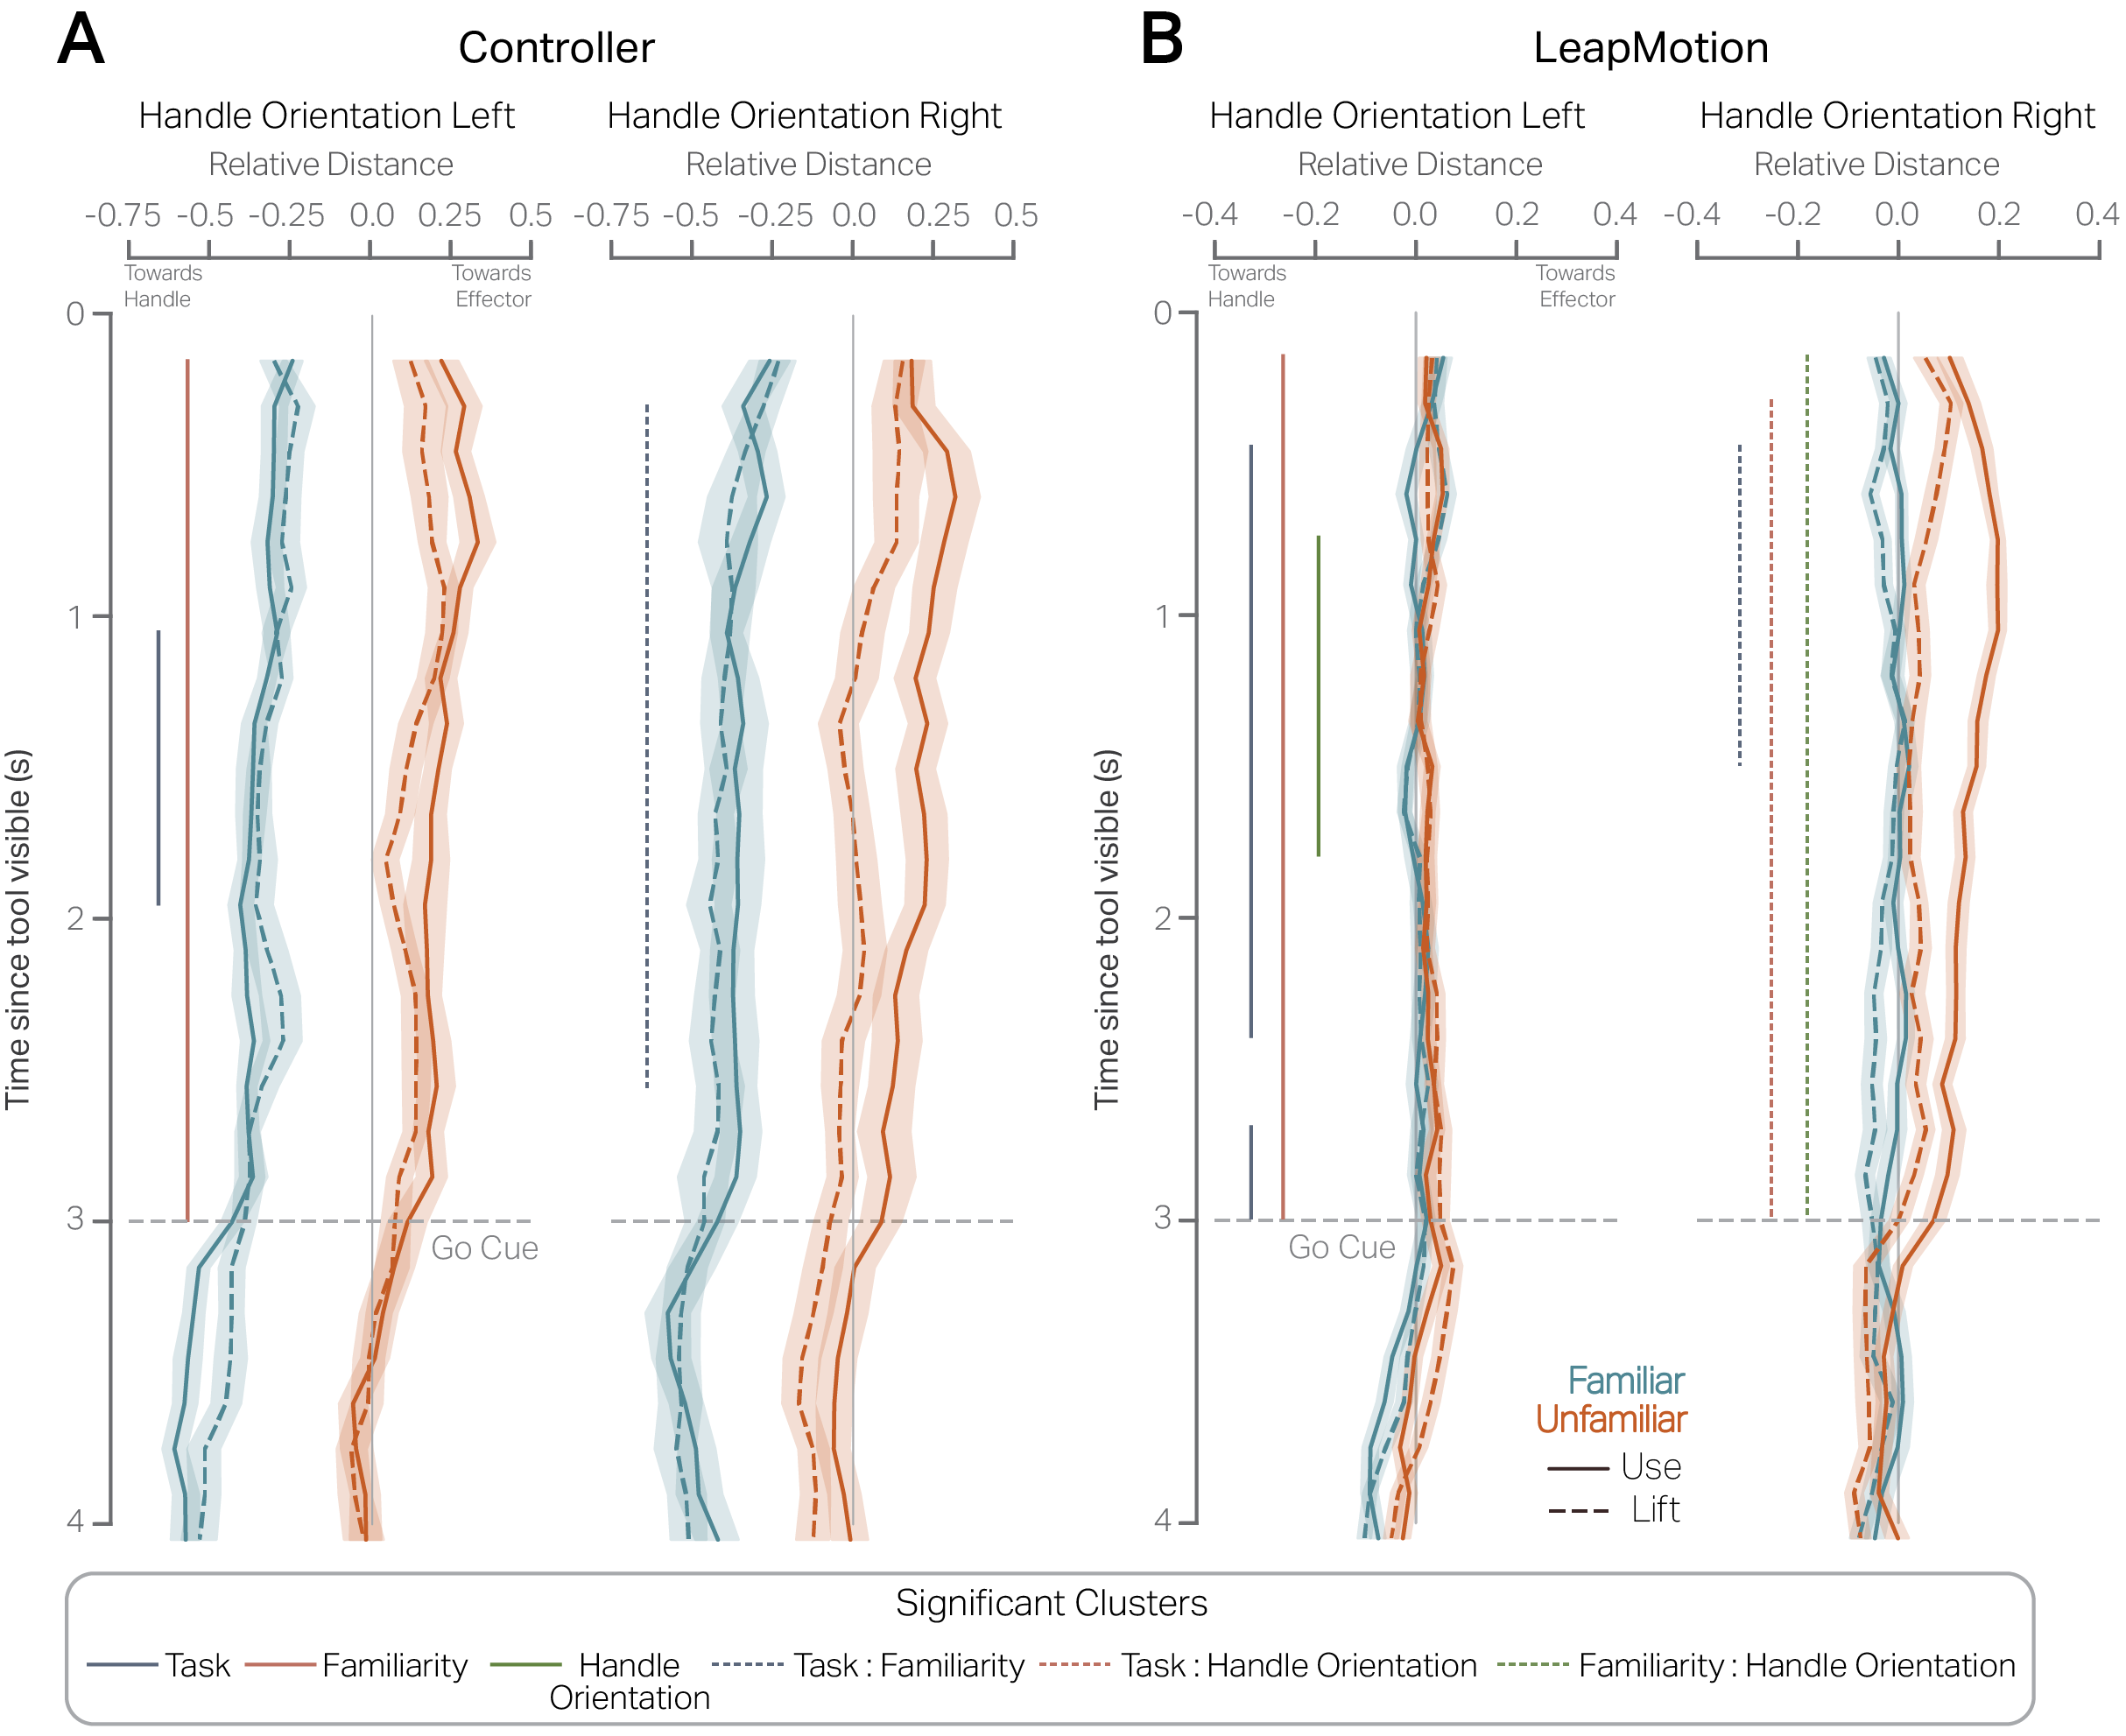
\includegraphics[width=1\linewidth]{source/figures/result/dev_center_final.png} \\
    \caption[]{Eccentricity of fixations on the tool models. The negative values of the abscissa correspond to fixations towards the handle, the positive values refer to fixations towards the tool effector, and zero represents the center of the tool. The ordinate axis refers to the time elapsed since the tool is visible on the virtual table. The go cue is given to participants at 3s after which they can start interacting with the tool. The blue lines correspond to the FAMILIAR tool and red to the UNFAMILIAR tools. The error bars represent the standard error of the mean across subjects.  The vertical solid lines correspond to the significant time clusters for main effects and the vertical dashed lines to the interactions. \textbf{Panel A} shows the findings from experiment-I and the two handle orientations. \textbf{Panel B} shows the findings from experiment-II and the two handle orientations.
}
    \label{figure:dev_from_center}
\end{figure}

Next, we were interested in the effect of task, tool familiarity, and handle orientation on the eccentricity of the fixations on the tool before action initiation. We calculated the relative distance of fixations from the center of the tool in the 3s period when the subjects studied the tool. We used cluster permutation tests to evaluate the time periods when the effects of the different conditions were significant. As shown in Figure \ref{figure:dev_from_center}A, in experiment-I, the differences in task (USE - LIFT) were significant from 1.05s to 1.95s period, p-value<0.001. Differences in tool familiarity (FAMILIAR - UNFAMILIAR) were significant from 0.15s to 3s with a p-value <0.001. Moreover, the differences in the two orientations (LEFT - RIGHT) were not significant. The interaction of task and familiarity were significant from 0.3s to 2.55s, p-value=0.006. The interactions of task and handle orientation, and the interaction of handle orientation and tool familiarity were not significant in any time period.

Similarly, figure \ref{figure:dev_from_center}B shows the eccentricity of fixations from the center of the tool during the 3s period when the subjects studied the tool in experiment-II. The differences in task were significant in two time periods 0.45s to 2.4s, p-value< 0.001 and from 2.7s to 3s, p-value=0.03. The differences in familiarity were significant from 0.15s to 3s, p-value < 0.001. Furthermore, the differences in handle orientation were significant from 0.75s to 1.8s, p-value < 0.001. A significant interaction of task and familiarity from 0.45s to 1.5s with p-value <0.001. There were also significant clusters in the interaction of task and handle orientation, from 0.3s to 3s with p-value<0.001 and for tool familiarity and handle orientation from 0.15s to 3s with p-value < 0.001.



